\documentclass[UTF8,a4paper]{ctexart}
%\usepackage[UTF8]{ctex}
\usepackage{graphicx}
\usepackage{url}
\usepackage{geometry}
\geometry{a4paper,scale=0.8}
\usepackage{setspace}
\setstretch{1.6}

\begin{document}
\begin{sloppypar}


	\begin{center}
	
\includegraphics[width = 14cm]{picture/s1}

		\begin{fontsize}{60pt}{20pt}
			实验报告
		\end{fontsize}

		\bigskip
		\bigskip
		
		\begin{fontsize}{20pt}{20pt}
			\begin{flushright}
				—— {\Huge Shell}与{\Huge Vim}的学习与应用
			\end{flushright}
		\end{fontsize}
		
		\bigskip
		\bigskip
		\bigskip
		\bigskip
		\bigskip
		\bigskip
		\bigskip
		\bigskip
		\bigskip
		\bigskip
		\bigskip
		\bigskip
		\bigskip
		\bigskip
		\bigskip
		\bigskip
		
		\begin{fontsize}{25pt}{20pt}

			学号:
			\underline{{\huge 23090013035}}
			\bigskip
			\bigskip
			\bigskip
			\bigskip

			姓名:
			\underline{朱永基}
			\bigskip
			\bigskip
			\bigskip
			\bigskip

			班级:
			\underline{{\Huge 23}级工程管理}
				
		\end{fontsize}
	\end{center}
	\section{实验要求}
	\subsection{学习Shell和Vim的使用}
	\subsection{完成4个课堂练习与20个与Shell和Vim有关的实例}

			\bigskip
			\bigskip
			\bigskip
			\bigskip

	\section{实验内容}
	\subsection{Shell的学习}
	\subsubsection{Shell 是一种命令行解释器和脚本编写环境,主要用于与操作系统的内核进行交互。它作为用户与操作系统之间的接口,允许用户输入命令并执行系统功能。Shell 可以理解并执行用户输入的命令,将它们传递给操作系统的内核,然后将结果返回给用户。\\Shell 通常以文本的形式运行,可以通过命令行终端访问。在 UNIX 和类 UNIX 系统(如 Linux 和 macOS)中,shell 是一个非常重要的工具,它允许用户执行各种系统管理任务、文件操作、网络配置等。\\常见的Shell类型有Bash、Zsh、Fish、Csh、Ksh。}
	\subsubsection{Shell的主要功能:\\1.命令解释: 接受用户输入的命令并传递给操作系统执行。\\2.脚本编写: 通过编写 Shell 脚本,用户可以自动化一系列操作,比如文件管理、系统监控、任务调度等。\\3.变量管理: Shell 允许用户创建和使用变量,以便在脚本中存储和操作数据。\\4.管道与重定向: 通过管道将一个命令的输出作为另一个命令的输入,或者通过重定向 控制输入输出。\\5.进程管理: Shell 可以启动、停止、后台运行进程,并管理系统资源的分配。}
	\subsubsection{Bash的核心功能:\\变量和参数: 在 Bash 中,变量可以通过 = 进行赋值,使用时通过 \$ 符号引用。\\Bash 支持条件语句和循环,如if-else,for循环等。\\函数: 可以在 Bash 中定义和调用函数,以实现代码的复用和模块化。\\管道:通过 \textbar 将一个命令的输出传递给另一个命令。\\重定向:将命令输出重定向到文件。}
	
	\newpage
	
	\subsection{Vim的学习}
	\subsubsection{Vim(Vi Improved)是一个功能强大、广泛使用的文本编辑器,特别在程序员和系统管理员中很受欢迎。它是经典编辑器 Vi 的增强版,支持多种功能如语法高亮、插件扩展、脚本编写等。}
	\subsubsection{Vim的特点:\\1.模式编辑:正常模式(Normal mode):用于浏览和编辑文件。按键直接影响光标移动和文本操作。插入模式(Insert mode):用于插入文本,类似于其他常见文本编辑器的编辑模式。可视模式(Visual mode):选择文本块进行操作(如复制、删除)。命令模式(Command mode):通过键入 : 来输入各种命令(如保存、退出等)。
\\2.高效的键盘操作: Vim 强调通过键盘进行操作,减少对鼠标的依赖,从而提高编辑效率。每个按键或按键组合都对应着一个特定的操作。\\3.强大的插件支持: Vim 有丰富的插件生态,可以通过插件扩展各种功能,如代码补全、文件树导航、Git 集成等。\\4.多平台支持: Vim 可以运行在不同的操作系统上,如 Linux、macOS 和 Windows,因此它被广泛用于跨平台的文本编辑。\\5.轻量级与可定制性: Vim 的配置非常灵活,可以通过 .vimrc 文件定制编辑器的行为、外观和功能。}
	

	\bigskip
	\bigskip
	\bigskip
	\bigskip
	\graphicspath{{picture/}}
	
	\newpage

	\section{实验中遇到的问题与解决方法}
	\subsection{在虚拟机中,从windows复制到linux中的脚本无法正常运行,错误提示: bash: ./1.sh: /bin/bash\^M: bad interpreter: No such file or directory}
	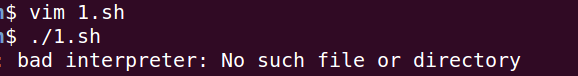
\includegraphics[width = 16cm]{q1}
	 这是由于文件中的换行符格式不正确引起的。具体来说,\^M 表示文件使用的是 Windows 风格的换行符(即 CRLF),而不是 Linux 期望的 Unix 风格的换行符(即 LF)。\\查阅资料后,下载并使用dos2unix命令,转变为Unix格式。\\
	 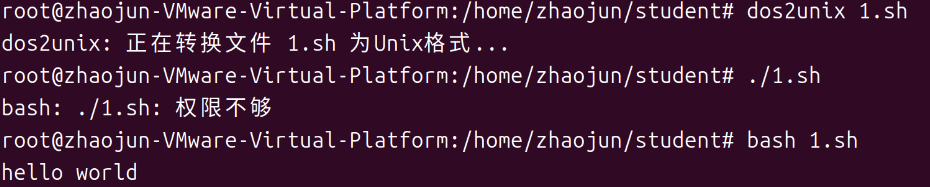
\includegraphics[width = 16cm]{q2}

	
			\bigskip
			\bigskip
			\bigskip
			\bigskip
			
	
	\section{实例练习}
	\subsection{查看历史命令}
	输入history命令,可以查看历史输入的所有命令
	
	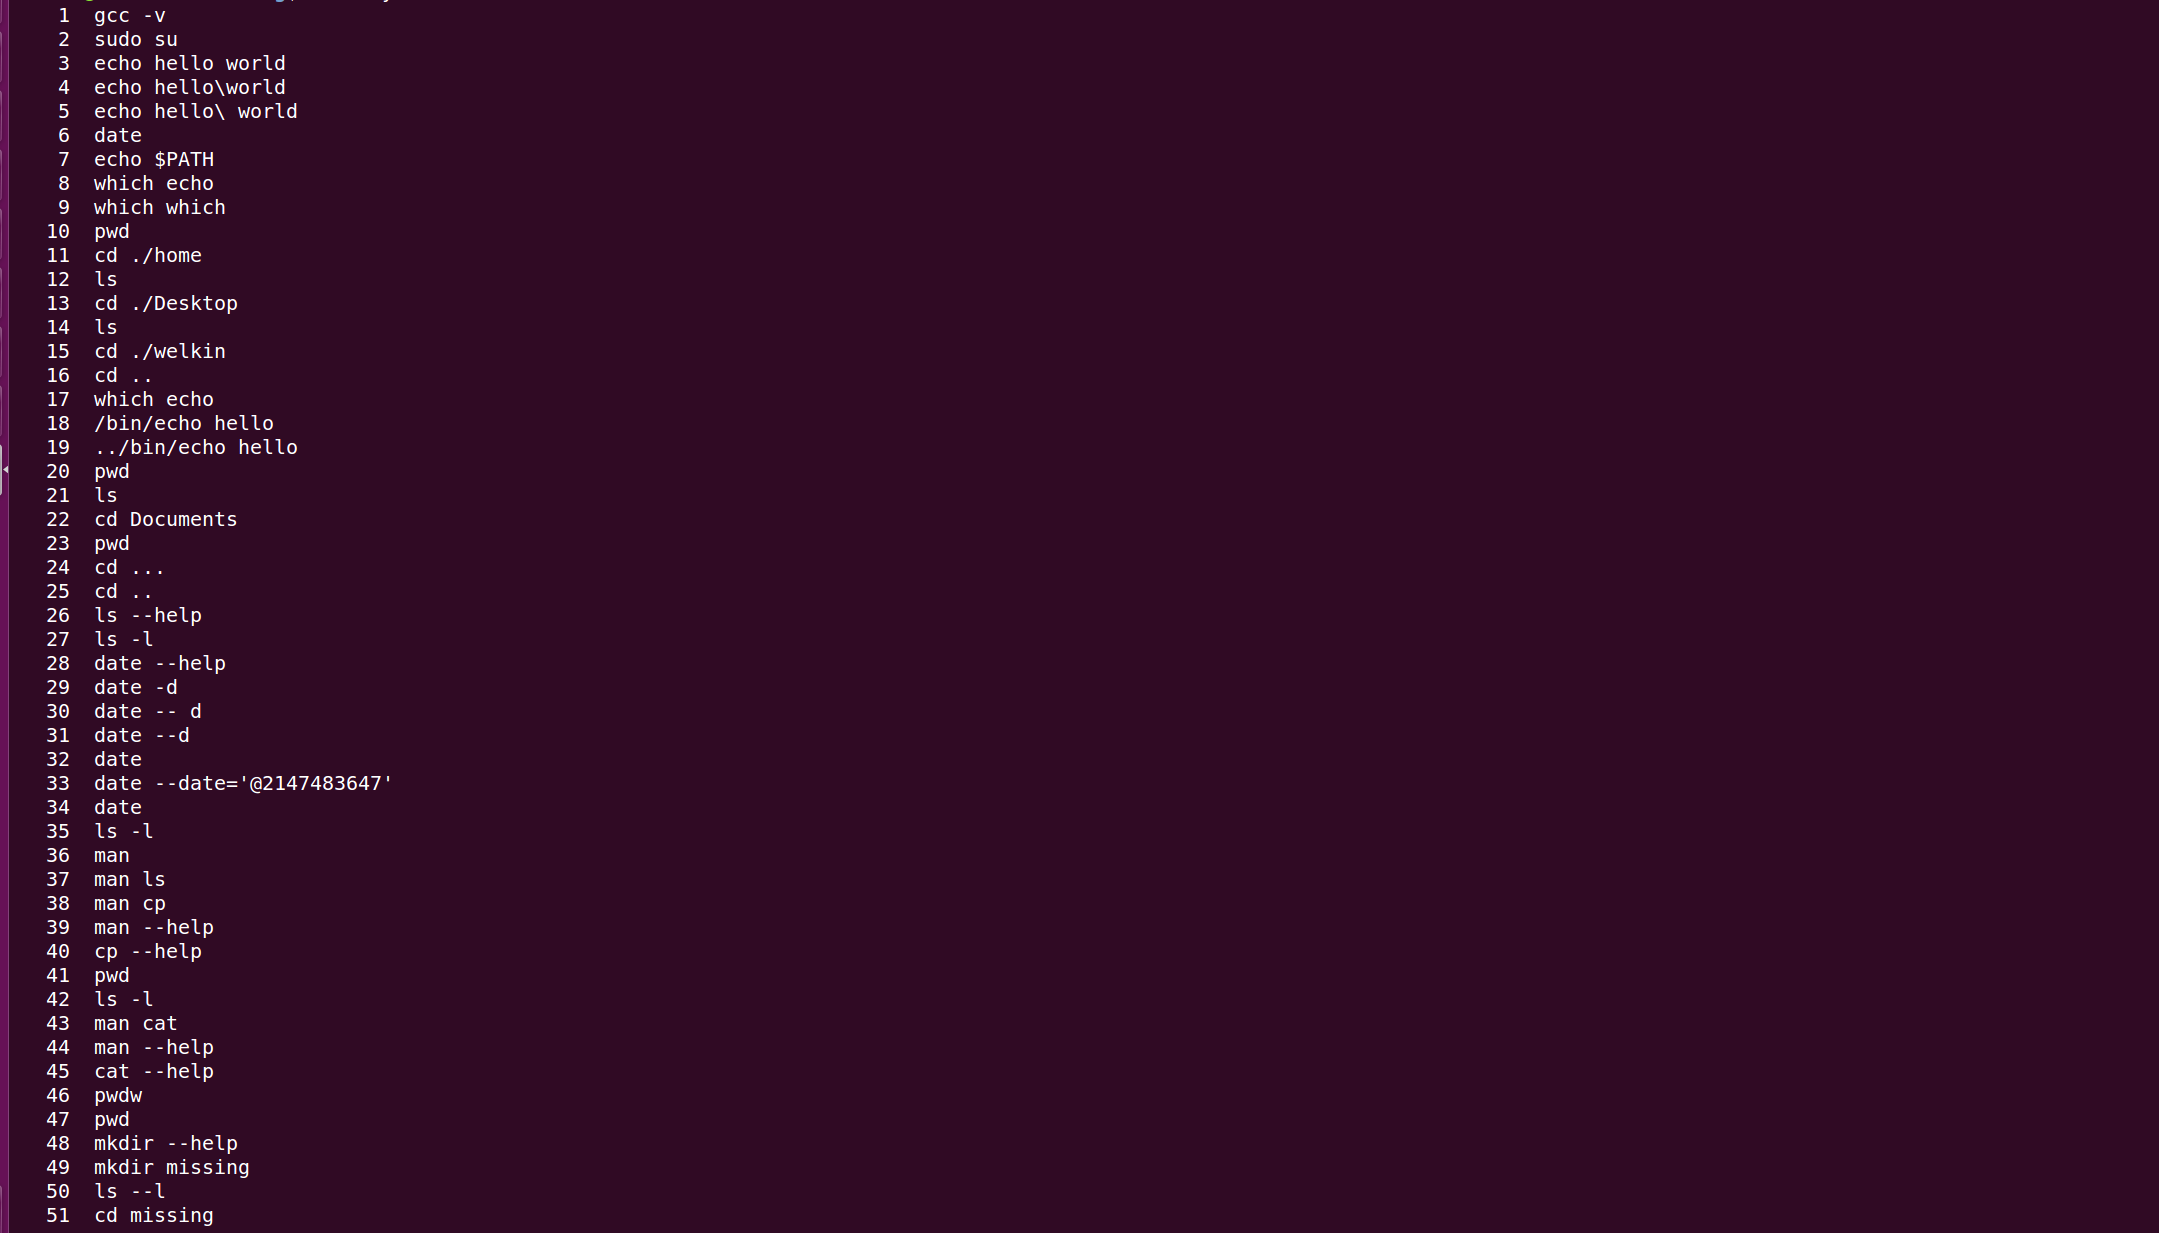
\includegraphics[width = 16cm]{1}
	
	\subsection{查看命令所在文件路径}
	输入which + xx 命令,即可显示命令所在文件路径
	
	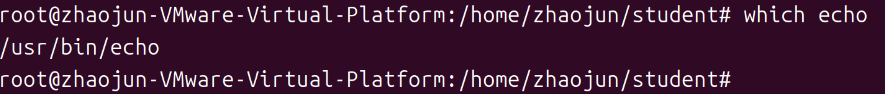
\includegraphics[width = 16cm]{2}
	
	\subsection{安装tldr命令}
	使用sudo apt-get install 等一系列操作,安装tldr命令为后面做准备
	
	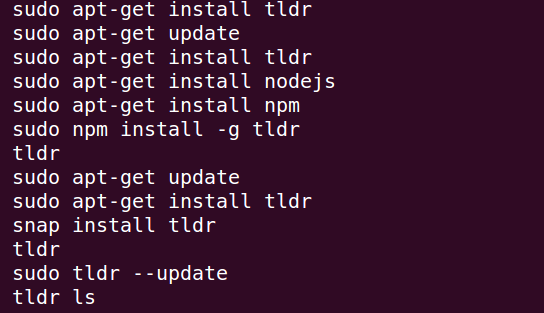
\includegraphics[width = 16cm]{3}
	
	\subsection{用tldr代替man}
	tldr意为太长不读,man的命令手册太长,tldr提供简略且有用的描述和使用案例
	
	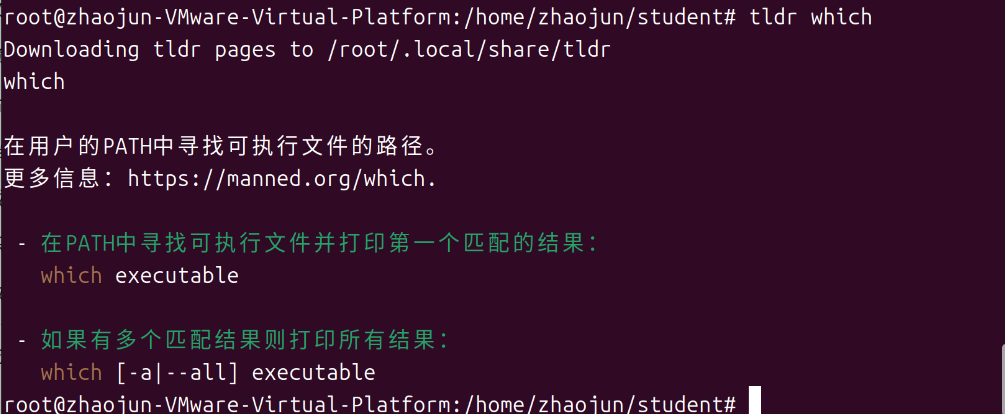
\includegraphics[width = 16cm]{4}
	
	\subsection{编写脚本函数}
	编写mcd脚本函数 \$1 是脚本的第一个参数,作用为创建并进入目录
	
	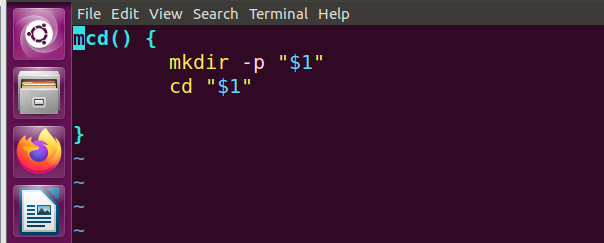
\includegraphics[width = 16cm]{5}
	
	\subsection{使用脚本中的函数}
	用source加载脚本,然后才可以使用里面的函数
	
	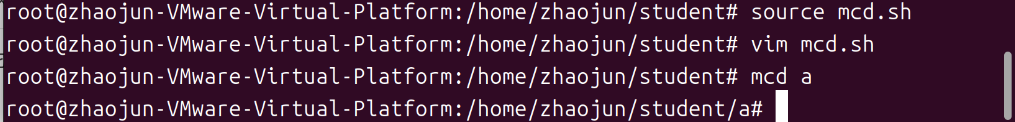
\includegraphics[width = 16cm]{6}
	
	\subsection{在文件中漫游}
	用ls,cd,pwd,mkdir等一系列命令漫游文件和目录
	
	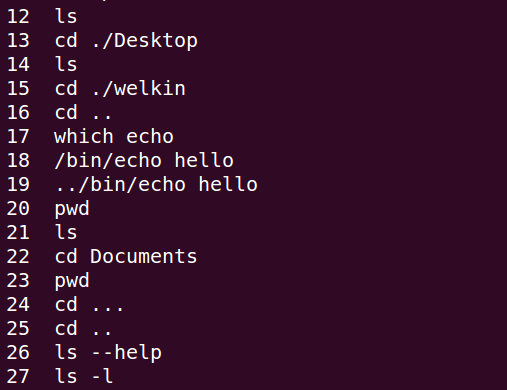
\includegraphics[width = 16cm]{7}
	
	\subsection{利用重定向复制文本内容}
	利用cat 和 重定向 > ,将一个文件的内容流到另一个文件中
	
	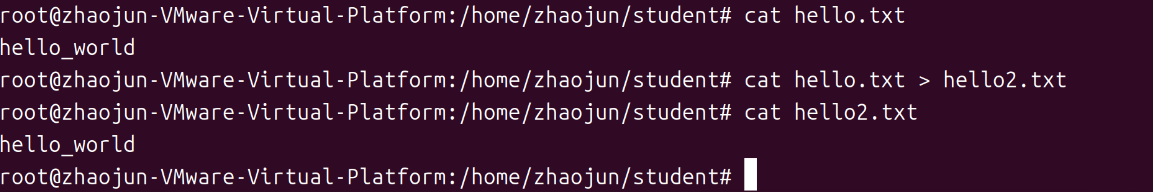
\includegraphics[width = 16cm]{8}
	
	\subsection{重定向控制输入输出}
	使用 > ,将原本输出到控制台的内容输出到world.txt中
	
	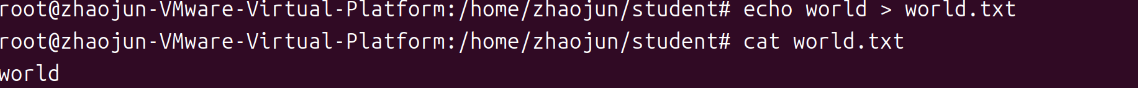
\includegraphics[width = 16cm]{9}
	
	\subsection{查看ls所有文件的最后一行}
	利用管道\textbar,沟通不同命令的输入和输出
	
	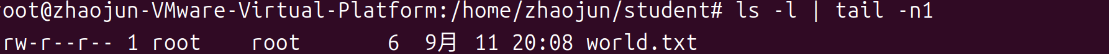
\includegraphics[width = 16cm]{10}
	
	\subsection{更好的查看目录结构}
	下载并使用tree命令,可以更美观的展示整体目录结构
	
	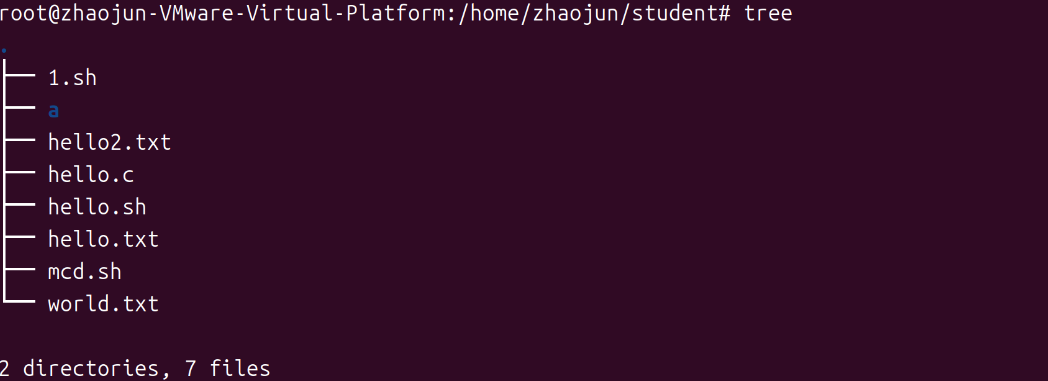
\includegraphics[width = 16cm]{11}
	
	\subsection{编写hello world脚本}
	在脚本中第一条包含shebang,实现一个简单的脚本
	
	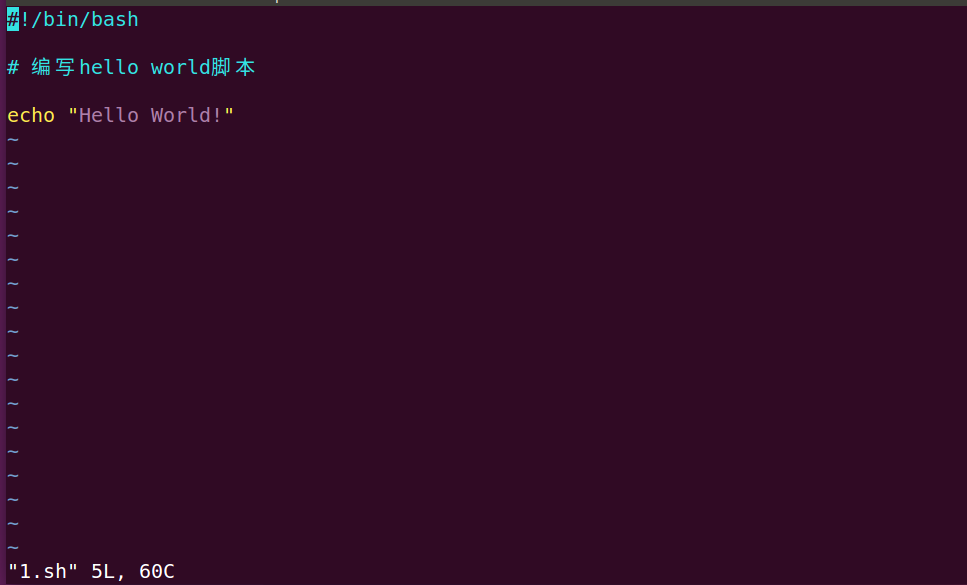
\includegraphics[width = 16cm]{12}
	
	\subsection{运行脚本}
	.表示上一级目录,采用相对路径运行脚本,成功输出hello world!
	
	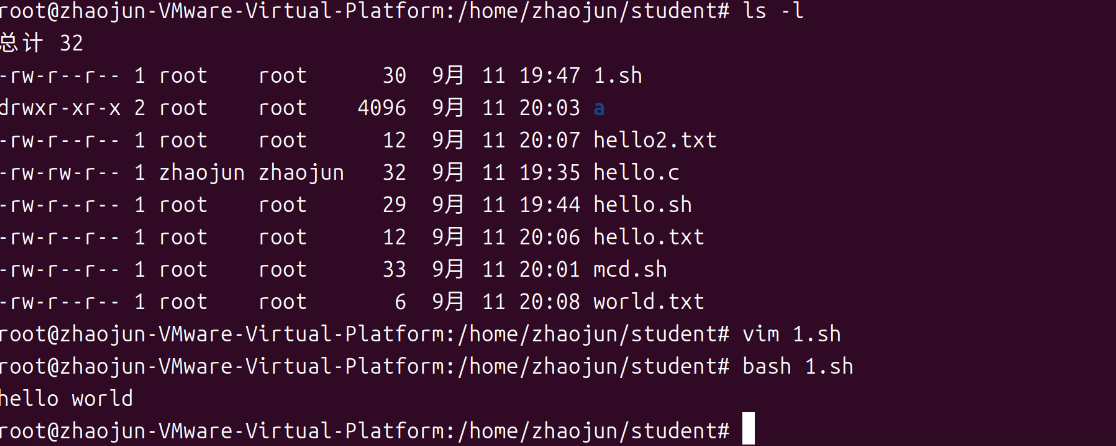
\includegraphics[width = 16cm]{13}
	
	\subsection{实现猜数字脚本}
	用while,if等实现一个简单的猜数字游戏,RANDOM 为系统自带的系统变量,值为 0‐32767的随机数,用取余使其变为1-100
	
	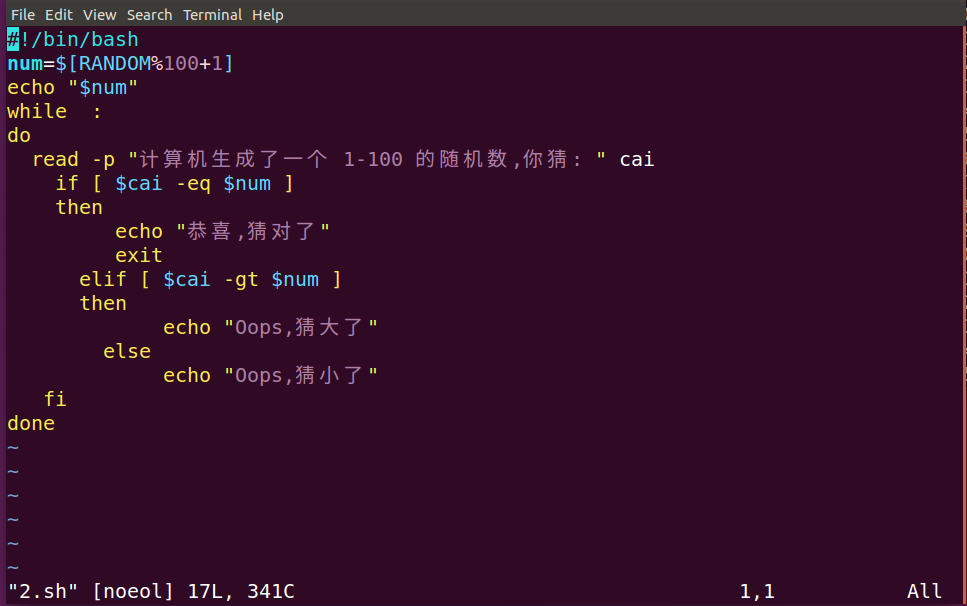
\includegraphics[width = 16cm]{14}
	
	\subsection{运行猜数字小游戏}
	不断读取数字直到猜中为止
	
	
\includegraphics[width = 16cm]{15}
	
	\subsection{vim显示buffer并切换}
	:buffers显示buffer,:bnext切换buffer,buffer犹如牌桌上叠放的两张牌,切换是让牌放在顶端
	
	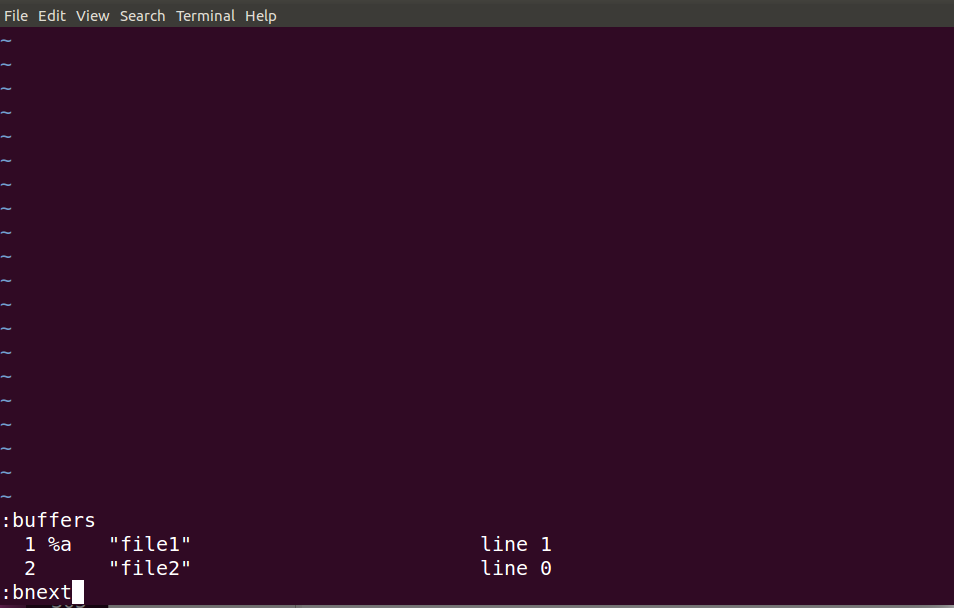
\includegraphics[width = 16cm]{16}
	
	\subsection{vim显示多个窗口}
	用:split + 文件名可以切割多个窗口并显示
	
	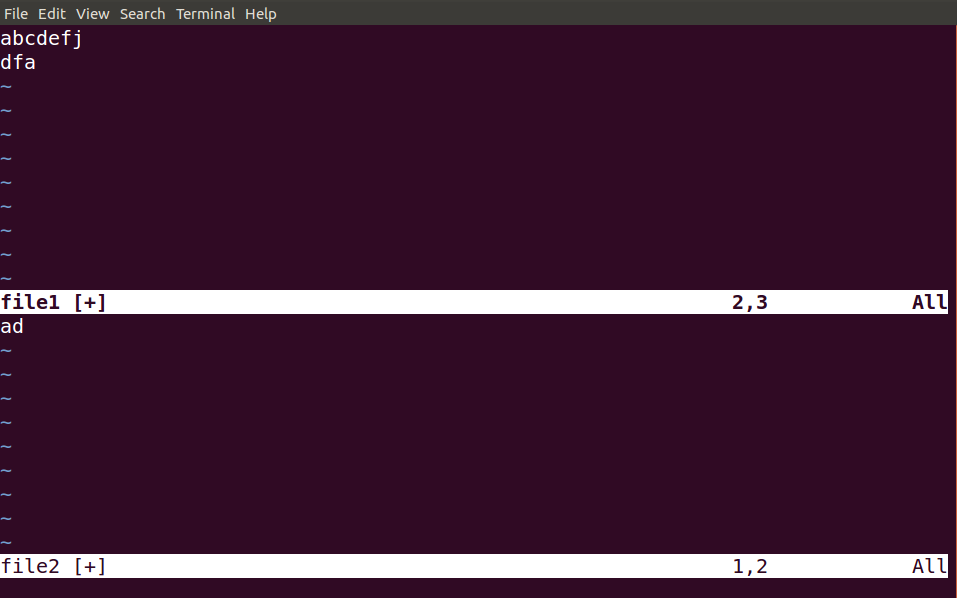
\includegraphics[width = 16cm]{17}
	
	\subsection{vim实现tabs}
	用:tabnew + 文件名,可以在新tab中打开文件
	
	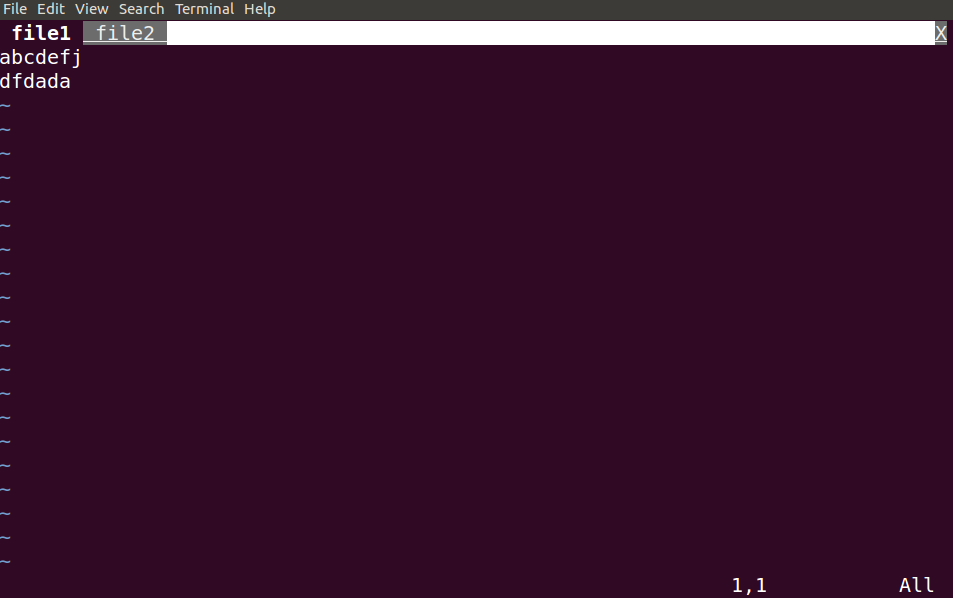
\includegraphics[width = 12cm]{18}
	
	\subsection{在vim中打开其他文件}
	:edit + 文件名,打开其他文件,这个文件属于新的buffer
	
	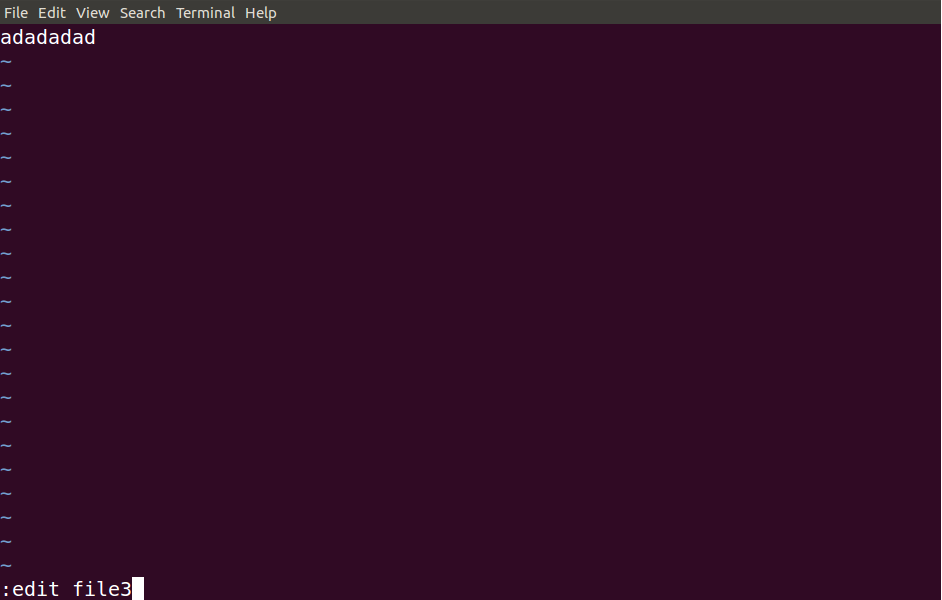
\includegraphics[width = 16cm]{191}
	
	\subsection{在vim中搜索文件内容}
	使用内置查找命令:vim /pattern/ file,查找含有相关文字的文件,按下enter则会进入相关文件
	
	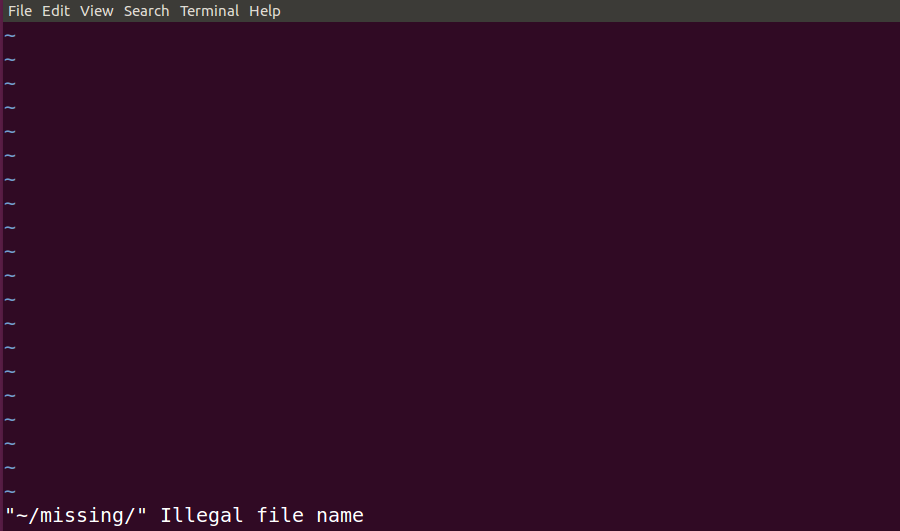
\includegraphics[width = 16cm]{201}

	\section{实验收获与感悟}
	学习 Shell 编程中的 Bash 和 Vim 编辑器是掌握 Linux 操作系统和自动化脚本开发的重要基础。我体会到了Bash脚本的强大和灵活性,如自动化工作流程,丰富的命令工具,条件语句与循环控制等;还有vim的高效编辑技巧,如高效的键盘操作,自定义与扩展,学习曲线陡峭但是回报丰厚!\\
	\indent 组合使用Vim和Bash,让我在Linux中游刃有余,同时学习Vim的过程也加深了对Shell环境的理解,如通过 Shell 命令调用 Vim 编辑文件、在 Vim 中直接执行 Shell 命令等。这种高效的命令行操作提升了整体的工作效率。同时促进了我在思维模式上的改变,学习 Bash 后,意识到重复性任务可以通过简单的脚本实现自动化,极大地解放了双手。同时,也让自己在面对问题时,更加倾向于寻找简洁的解决方案。\\
	\indent 学习 Bash 和 Vim 后,最大的感悟是提升了自己的工作效率和自动化能力,尤其是在 Linux 环境下的操作更加得心应手。同时,这种学习过程培养了自己高效处理问题、精益求精的习惯,并进一步提升了自己的编程思维和脚本开发技能。\\
	
	Github仓库链接:\url{https://github.com/zhaojun262510/program1}
	
\end{sloppypar}
\end{document}